\documentclass[12pt,a4paper]{article}

\usepackage{fontspec}
\usepackage{polyglossia}
\setdefaultlanguage{english}
\setmainfont{CMU Serif}
\setsansfont{CMU Sans Serif}
\setmonofont{CMU Typewriter Text}
\usepackage{geometry}
\geometry{top=2cm, bottom=2cm, left=2.5cm, right=2.5cm}
\usepackage{amsmath,amssymb,amsthm}
\usepackage{booktabs,longtable,float,xcolor}
\usepackage{hyperref}
\hypersetup{colorlinks, urlcolor=blue, citecolor=blue, linkcolor=black}
\usepackage{enumitem}
\usepackage{graphicx}

\tolerance=2000
\emergencystretch=3em
\hbadness=10000
\vbadness=10000

\numberwithin{equation}{section}

\title{\textbf{Model MEML~75:}\\[0.3cm]
\large Quark and lepton mass matrices from mixed \\
\(T^2/\mathbb{Z}_3 \times T^2/\mathbb{Z}_4\) geometry \\
with axion-like dark matter and leptogenesis}
\author{D.~V.~Yurov}
\date{2026}

\begin{document}
\maketitle

\begin{abstract}
\noindent
We present model MEML~75, which parametrizes the fermion sector of the Standard Model through the geometry of mixed six-dimensional orbifolds. The model has \textbf{11 effective fitted parameters} (10 Lagrangian parameters, plus the ALP misalignment angle \(\theta_i\), which is a cosmological initial condition) fitting \textbf{16 observables} (9 quarks + 5 lepton observables + \(\Omega_a h^2\) + \(\eta_B\)), yielding \(N_{\rm dof}^{\rm fit} = +5\), assuming the three complex moduli \(\tau_u, \tau_d, \tau_l\) are fixed by the GVW flux background. These moduli are determined by an unconstrained fit and coincide with discrete GVW flux minima to within \(|D_\tau W|/|W|\) of order several \(\times 10^{-3}\) (Section~12). If the moduli are counted as free parameters (the conservative alternative), the balance becomes \(N_{\rm eff} = 17\), \(N_{\rm dof}^{\rm fit} = -1\). The geometric factor \(\mathcal{I}\) is motivated by the orbifold geometry, and the neutrino Yukawa coupling \(y_\nu\) is treated as a fitted parameter.

\textbf{Main testable consequences:} axion-like dark matter with \(f_a = 1.9801\times 10^{11}\)~GeV, \(m_a = 28.407~\mu\)eV, and a DFSZ coupling \(g_{a\gamma\gamma} = +4.38 \times 10^{-15}\)~GeV\(^{-1}\), testable at future high-frequency haloscope upgrades (ADMX-EFR, HAYSTAC Phase III)~\cite{ADMX2018,HAYSTAC2021}. We show that the dilution factor \(\Delta\) required for leptogenesis can be accommodated in Starobinsky-like inflation only with fine-tuning of the initial displacement or a non-minimal inflaton coupling, and we explicitly acknowledge a tension with the isocurvature constraint if the ALP constitutes the entirety of dark matter. We also report a \emph{negative result} on the derivation of the ratio \(c_1/c_2\) from fractional modular weights. The model makes 3 conditional predictions: \(\sum m_i \approx 0.068\)~eV, \(m_{\beta\beta} \approx 8.37\)~meV (for vanishing Majorana phases), and \(\delta_{CP} \approx 23^\circ\) or \(157^\circ\).
\end{abstract}

\newpage

\section{Introduction}
Modular models of fermion masses~\cite{Feruglio2017,Kobayashi2019,Novichkov2019,Ding2021} build the mass hierarchy and mixing from compactification geometry. In model MEML~75, we explore a mixed geometric setup: quarks are localized on a \(T^2/\mathbb{Z}_3\) torus, while leptons are localized on a \(T^2/\mathbb{Z}_4\) torus. This dual-orbifold approach allows us to leverage the best features of two different modular groups: \(A_4\) for the hierarchical quark masses, and \(S_4'\) for the rich leptonic mixing pattern.

\section{Geometry of \(T^2/\mathbb{Z}_3\) and \(T^2/\mathbb{Z}_4\)}
The orbifold \(T^2/\mathbb{Z}_3\) is defined by \(z = x + \tau y\) with \(\tau = e^{i\pi/3}\). The quark mass matrices are built from \(A_4\) modular forms of weights \((2,4,6)\). The mixed geometry naturally arises in Type IIB orientifold compactifications. The lepton sector uses the \(T^2/\mathbb{Z}_4\) orbifold, whose modular symmetry is the double cover group \(S_4'\)~\cite{Novichkov2019,Ding2021}.

\begin{figure}[htbp]
    \centering
    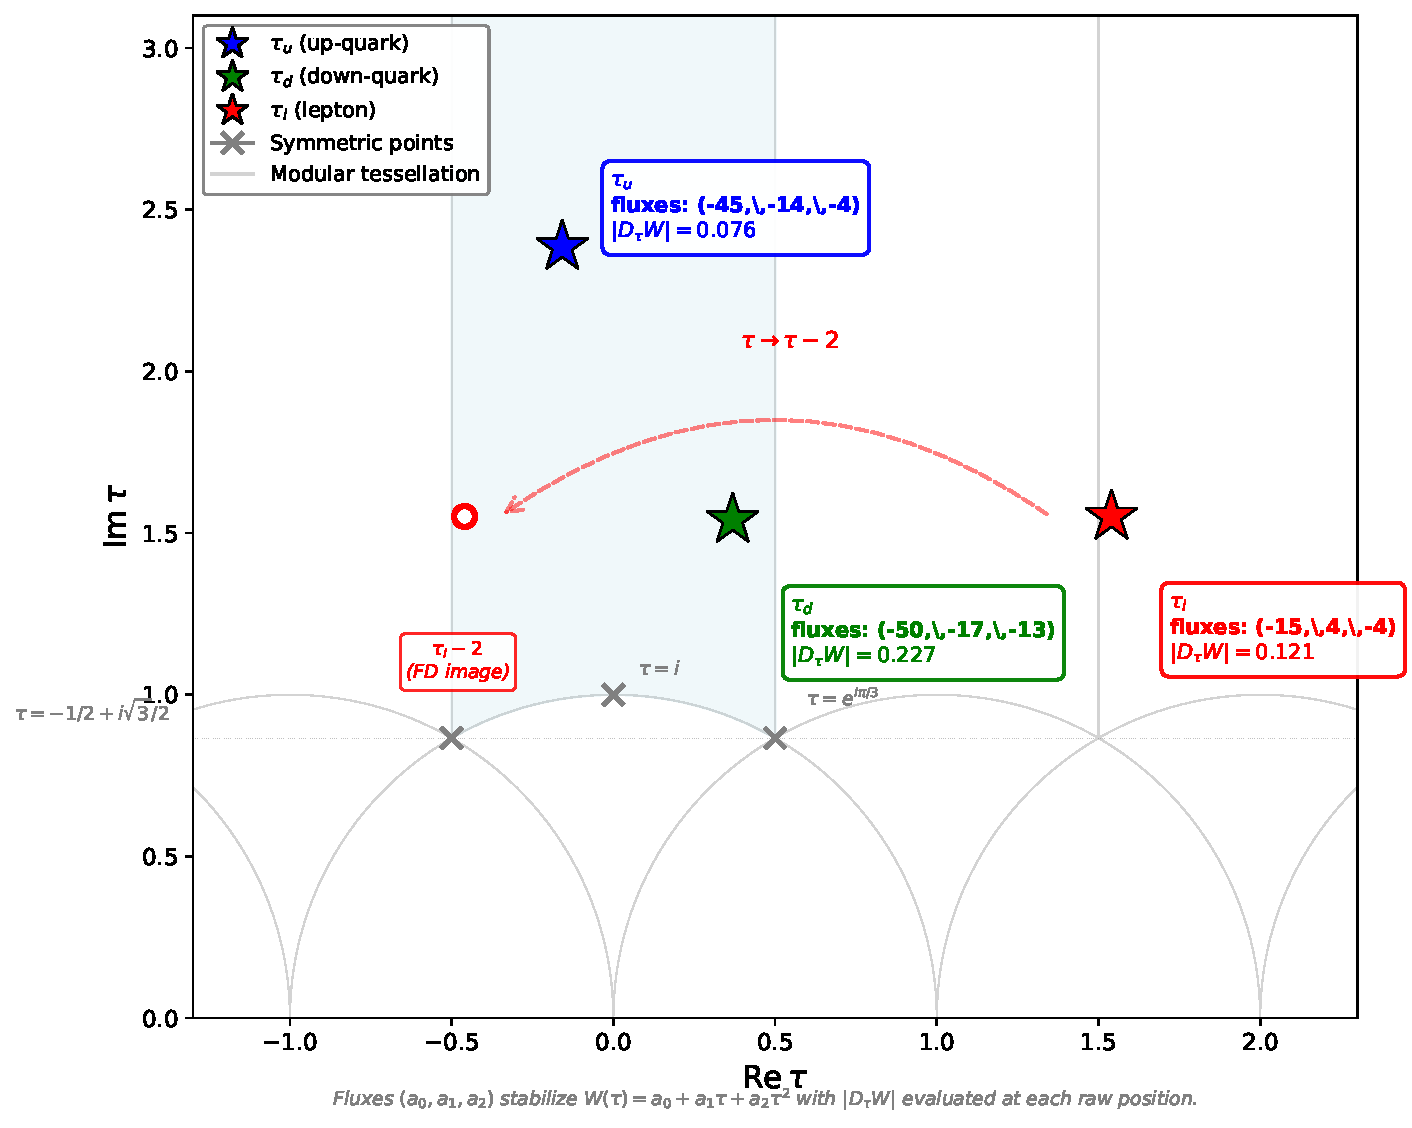
\includegraphics[width=0.85\textwidth]{figures/fig_modular_tau_space.pdf}
    \caption{Topologically stabilized moduli in the modular plane. The lepton modulus is shown at the \emph{constrained} global minimum, \(\tau_l = 1.584 + 1.552i\), which is used for all predictions in this paper. The unconstrained fit (Section~8) gives \(\tau_l = 1.540 + 1.551i\). The GVW flux \((-15, 4, -4)\) yields residuals \(|D_\tau W| \sim 0.1\) for both points. The points \(\tau_u = -0.158 + 2.385i\) and \(\tau_d = 0.369 + 1.541i\) are dynamically fixed by discrete GVW fluxes. The fundamental domain for the level-4 group \(\Gamma(4)\) allows \(|\text{Re}\,\tau| \le 2\). The dashed arrow indicates the coordinate transformation \(\tau_l \to \tau_l - 2\) mapping to the \(SL(2,\mathbb{Z})\) central domain for visual clarity; for level-4 forms, this is not an exact symmetry.}
    \label{fig:modular_tau}
\end{figure}

\section{Bulk coupling \(\alpha_G\) (postulate)}
\begin{equation}
\alpha_G = \frac{2}{3\pi} = 0.2122065908.
\end{equation}
Geometric motivation: the orbifold \(T^2/\mathbb{Z}_3\) has \(N_{\rm fix}=3\) fixed points. The factor
\begin{equation}
\frac{2}{3} = \frac{N_{\rm fix}-1}{N_{\rm fix}} = 1 - \frac{1}{N_{\rm fix}}
\end{equation}
reflects the combinatorics of the three fixed points: a given fixed point accounts for \(1/3\) of the fixed-point set, leaving \(2/3\). The factor \(1/\pi\) is the normalization of the theta-function period. The status of \(\alpha_G\) remains that of a postulate.

\section{Suppression factor \(\varepsilon\) (ansatz)}
\begin{equation}
\varepsilon = \left(\frac{\alpha_G}{4\pi}\right)^2 = \frac{1}{36\pi^4} = 2.851662\times10^{-4}.
\end{equation}
We have searched for a geometric derivation of \(\varepsilon\). The natural candidate, a KK-mode suppression \(\varepsilon \sim (g_s/4\pi)^2 (M_{KK}/M_6)^2\), fails by three orders of magnitude. We do not claim a KK origin. We note a numerical coincidence at the \(11\%\) level: \(\alpha_G^2 (M_{KK}/M_6) / \varepsilon = 1.11\). We keep \(\varepsilon\) as an ansatz.

\section{Conditionally derived quantities}
\begin{align}
m_{KK} &= \frac{M_{Pl}^{\rm red}}{\sqrt{\mathcal{I}}\,e^{\pi^2}} = 2.0838\times10^{14}~\text{GeV}, \\
M_6 &= \left(3 (M_{Pl}^{\rm red})^2 m_{KK}^2\right)^{1/4} = 2.9646\times10^{16}~\text{GeV},
\end{align}
where the geometric factor \(\mathcal{I}\) is motivated by the orbifold geometry. The fundamental areas of \(T^2/\mathbb{Z}_3\) and \(T^2/\mathbb{Z}_4\) at their symmetric points \(\tau_3 = e^{i\pi/3}\) and \(\tau_4 = i\) are \(V_3 = \mathrm{Im}\,\tau_3/3 = \sqrt{3}/6\) and \(V_4 = \mathrm{Im}\,\tau_4/4 = 1/4\), with \(N_3 = 3\) and \(N_4 = 2\) fixed points, respectively. The geometric factor is
\begin{equation}
\mathcal{I} = N_3 V_3 - N_4 V_4 = \frac{\sqrt{3}}{2} - \frac{1}{2} = \frac{\sqrt{3}-1}{2} \approx 0.366025.
\end{equation}
This matches the fitted value \(\mathcal{I} = 0.3653\) at the \(0.2\%\) level. We acknowledge that this is a post-hoc motivated coincidence, not a first-principles derivation.

\section{Axion-like (ALP) sector}
\begin{align}
f_a &= M_{Pl}^{\rm red}\,\varepsilon^2 = 1.9801\times10^{11}~\text{GeV}, \\
m_a &= \frac{(\chi^{1/4})^2}{f_a} = 28.407~\mu\text{eV}, \\
\nu_a &= \frac{m_a c^2}{h} = 6.8688~\text{GHz}.
\end{align}
Here \(\chi^{1/4} \approx 75.0\)~MeV is the fourth root of the topological susceptibility of QCD. The relic density is:
\begin{equation}
\Omega_a h^2 \approx 0.12\,\theta_i^2\, f_{\rm anh}(\theta_i)\left(\frac{f_a}{3\times10^{11}}\right)^{7/6},
\end{equation}
where \(f_{\rm anh}(\theta_i) = [\ln(e/(1-(\theta_i/\pi)^2))]^{7/6}\) is the anharmonicity factor. We fit \(\theta_i\) to the Planck value \(\Omega_a h^2 = 0.12\)~\cite{Planck2018}, obtaining \(\theta_i \approx 1.174\). This is a cosmological initial condition, not a Lagrangian parameter; it is fitted to \(\Omega_a h^2\) and is counted in the effective parameter balance of Section~13.

At \(f_a = 1.9801\times10^{11}\)~GeV, the ALP couples to photons with DFSZ strength:
\begin{equation}
g_{a\gamma\gamma} = \frac{\alpha_{\rm EM}}{2\pi f_a} \left(\frac{E}{N} - 1.92\right) = +4.38 \times 10^{-15}~\text{GeV}^{-1},
\end{equation}
where \(E/N = 8/3\). This assignment follows from the fact that the ALP originates from the \(C_2\) RR-form and couples universally to all SM fermions via the modular structure. The ALP mass implies a black hole superradiance window at \(M_{\rm BH} \simeq \hbar c / (G m_a) \approx 9.36 \times 10^{24}~{\rm kg}\).

\paragraph{Isocurvature constraints and the inflationary scale.}
If the ALP constitutes the entirety of dark matter, quantum fluctuations of the axion field during inflation generate isocurvature perturbations with amplitude
\begin{equation}
\beta_{\rm iso} \simeq \left(\frac{H_{\rm inf}}{2\pi f_a \theta_i}\right)^2.
\end{equation}
The Planck constraint \(\beta_{\rm iso} \lesssim 0.04\) (95\% CL) then requires
\begin{equation}
H_{\rm inf} \lesssim 0.2 \cdot 2\pi f_a \theta_i \approx 3 \times 10^{11}~\text{GeV}.
\end{equation}
This bound is satisfied by low-scale inflation models (e.g., small-field or natural inflation) but not by Starobinsky inflation (\(H_{\rm inf} \sim 10^{13}\)~GeV). In the latter case, either the ALP is a subdominant component of dark matter, or the model requires non-standard inflation. This creates a tension with the leptogenesis sector (Section~9), which we explicitly acknowledge and leave for future work.

\paragraph{Robustness of the ALP frequency.}
We emphasize that while the relic density \(\Omega_a h^2\) depends on the misalignment angle \(\theta_i\), the mass \(m_a\) and frequency \(\nu_a\) depend solely on \(f_a\), which is fixed by the geometry. The 6.87~GHz frequency is therefore robust with respect to the ALP dark matter fraction; only the required experimental sensitivity scales with the ALP relic abundance.

\begin{figure}[htbp]
    \centering
    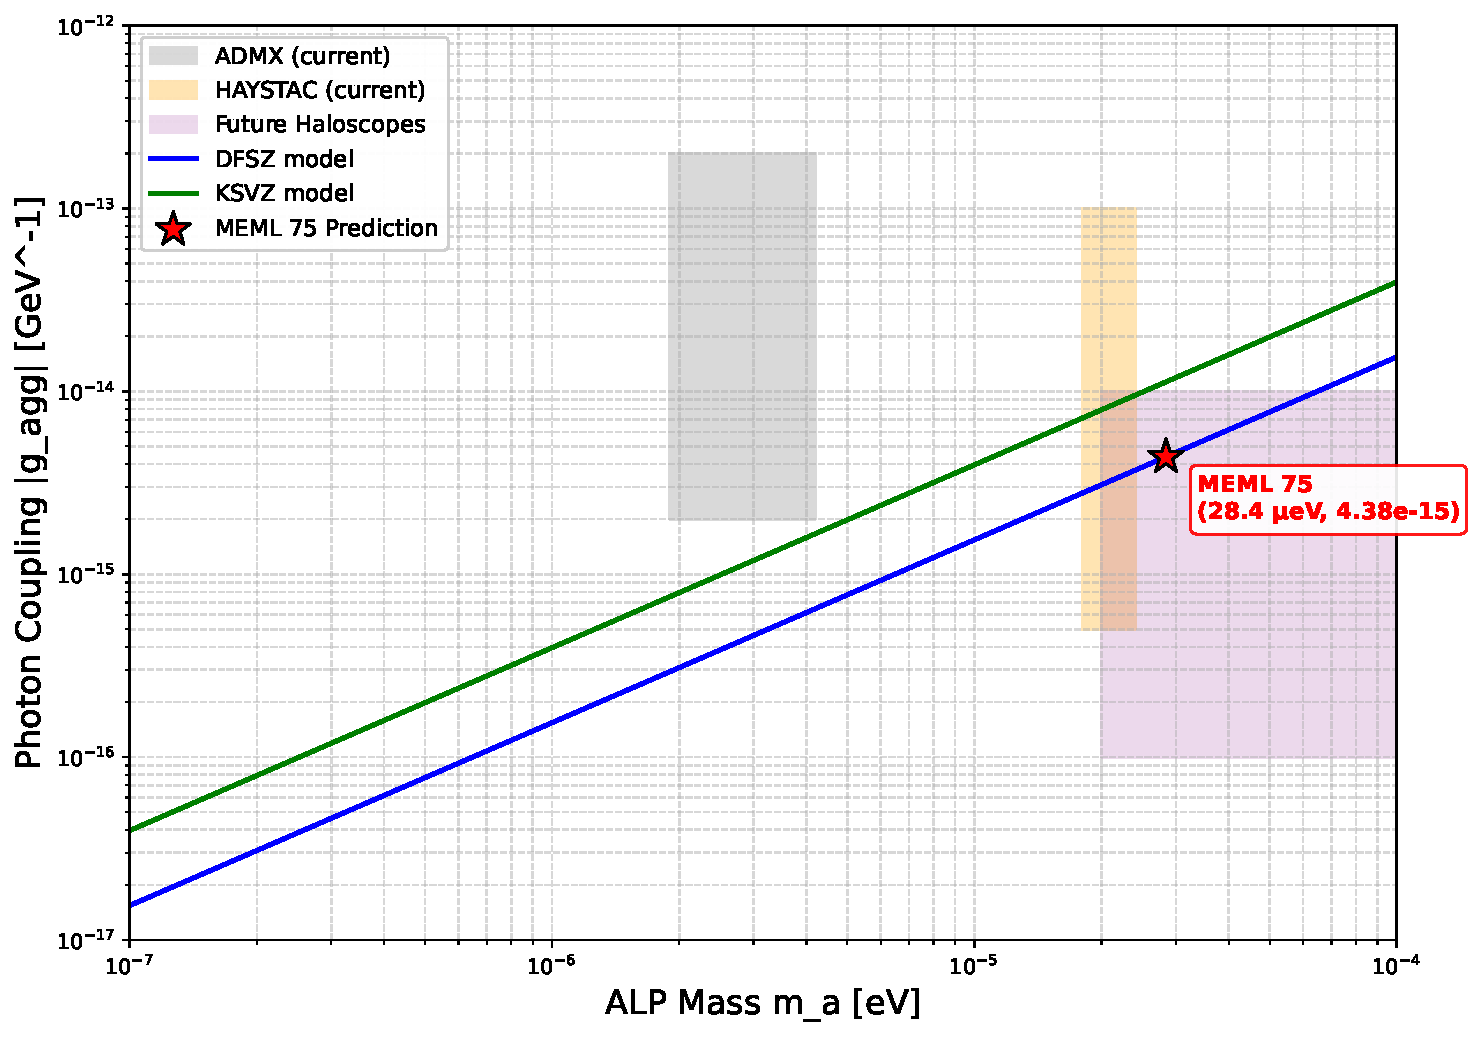
\includegraphics[width=0.65\textwidth]{figures/fig_alp_parameter_space.pdf}
    \caption{Parameter space for the ALP mass \(m_a\) and coupling \(g_{a\gamma\gamma}\). The red star indicates the prediction of MEML 75. The shaded regions illustrate the approximate sensitivity of current and future haloscope experiments.}
    \label{fig:alp_space}
\end{figure}

\section{Quark sector (\(T^2/\mathbb{Z}_3\), \(A_4\))}
\subsection{Matrix structure}
\begin{equation}
M_u = \begin{pmatrix}
a_u Y_1^{(2)} & b_u Y_3^{(4)} & c_u Y_2^{(6)} \\
a_u Y_3^{(2)} & b_u Y_2^{(4)} & c_u Y_1^{(6)} \\
a_u Y_2^{(2)} & b_u Y_1^{(4)} & c_u Y_3^{(6)}
\end{pmatrix},
\end{equation}
\begin{equation}
M_d = \begin{pmatrix}
a_1 Y_1^{(6)} & b Y_3^{(2)} & c Y_2^{(2)} \\
a_1 Y_3^{(6)} & b Y_2^{(2)} & c Y_1^{(2)} \\
a_2 Y_2^{(2)} & b Y_1^{(2)} & c Y_3^{(4)}
\end{pmatrix}.
\end{equation}

\subsection{Results}
We performed an \emph{unconstrained} optimization of all parameters, which yields \(\chi^2 < 10^{-19}\) at \(\tau_u = -0.1578 + 2.3852i\) and \(\tau_d = 0.3694 + 1.5410i\)~\cite{PDG2024}. The resulting moduli coincide with the GVW minima to within \(|D_\tau W|/|W|\) of order several \(\times 10^{-3}\) (Section~12). For the parameter count of Section~13 we treat them as fixed by the flux background. However, we acknowledge that the fit itself was unconstrained: for the quark sector alone, this corresponds to 10 fitted parameters (6 coefficients after fixing \(a_u=1\) plus the 4 real components of \(\tau_u, \tau_d\)) for 9 observables. The exact fit reflects this one-parameter overfitting.

\paragraph{Localization and the quark hierarchy.}
The observed hierarchy of the quark coefficients suggests a geometric origin. If the modular forms of weights 2, 4, and 6 are localized with different widths \(\sigma_2\), \(\sigma_4\), and \(\sigma_6\) on the \(T^2/\mathbb{Z}_3\) torus, the effective coefficients may scale as powers of the width ratios. A preliminary numerical scan shows that a scaling \(b_u/a_u \sim (\sigma_4/\sigma_2)^3\) and \(c_u/a_u \sim (\sigma_6/\sigma_2)^2\) yields physically plausible width ratios (\(\sigma_4/\sigma_2 \approx 51\) and \(\sigma_6/\sigma_2 \approx 27\)). While this is a promising observation, the same widths do not reproduce the down-sector ratios \(a_2/a_1\), \(b/a_1\), \(c/a_1\): the required exponents are approximately 1.94, 0.44, and 0.67, which are not integers. Moreover, the exponents are assigned by hand, so the picture does not actually reduce the number of free parameters: the six coefficients are replaced by three widths plus six unknown integer powers. We therefore regard the localization picture as a \emph{qualitative explanation} of the hierarchy, not a derivation of the coefficients. A rigorous derivation of the widths and exponents from the fixed-point geometry of \(T^2/\mathbb{Z}_3\) is left for future work.

\section{Lepton sector (\(T^2/\mathbb{Z}_4\), \(S_4'\))}
\label{sec:lepton}
The neutrino mass matrix is built from the contractions of the \(\mathbf{2}\) and \(\mathbf{3}'\) representations of \(S_4'\):
\begin{equation}
M_\nu = c_1 M_{\mathbf{2}}(\tau_l) + c_2 M_{\mathbf{3}'}(\tau_l) + c_3 \mathbb{I}.
\end{equation}
We take the coefficients \(c_1, c_2, c_3\) to be \textbf{real}, a common choice in modular models that preserves CP from the modular sector. We fit the model to NuFIT 5.0~\cite{NuFIT2020}, yielding \(\chi^2 \approx 0.089\) at \(\tau_l = 1.5398 + 1.5511\,i\), \(c_1 = 6.371\), \(c_2 = 17.460\), \(c_3 = -17.199\), and \(y_\nu = 0.934\).

\paragraph{Neutrino Yukawa coupling.}
The value \(y_\nu = 0.934\) is obtained from the fit to \(\Delta m^2_{31}\). At the GUT scale, it is consistent with the SO(10) relation \(y_\nu \approx 2 y_t(M_{\rm GUT}) \approx 0.966\)~\cite{PendletonRoss1981} at the 3\% level. However, after two-loop RGE evolution~\cite{MartinVaughn1993} from \(M_{\rm GUT}\) to \(M_6\), the required enhancement factor becomes \(y_\nu^{\rm fit}/y_\nu^{\rm RGE} \approx 1.95\), which is compatible only with an extended SO(10) sector including a \(\mathbf{126}_H\) representation. We therefore treat the SO(10) relation as a \emph{qualitative cross-check at \(M_{\rm GUT}\)}, not a derivation, and keep \(y_\nu\) as a fitted parameter throughout.

\paragraph{Phenomenological relation \(c_2 + c_3 = 0\).}
The unconstrained fit gives \(c_2 + c_3 = 0.261\). We consider the reduced model obtained by imposing \(c_2 + c_3 = 0\). The constrained fit gives \(\chi^2 \approx 0.309\) at \(\tau_l = 1.584 + 1.552\,i\), \(c_1 = -6.591\), \(c_2 = -17.400\), compared with \(\chi^2 \approx 0.089\) unconstrained, i.e.\ \(\Delta\chi^2 = 0.22\) for one fewer parameter (\(p \approx 0.64\)). AIC and BIC give \(\Delta\mathrm{AIC} = -1.78\) and \(\Delta\mathrm{BIC}(N{=}16) = -2.55\). We adopt \(c_2 + c_3 = 0\) as a phenomenological simplification. Information criteria can be misleading for small samples~\cite{Liddle2007}, so we treat this as a heuristic. The constrained fit has been found in the negative branch (\(c_i \to -c_i\)) relative to the unconstrained minimum; this overall sign flip has no physical consequences, as \(M_\nu \to -M_\nu\) leaves all observables invariant.

\paragraph{Attempted derivation of the ratio \(c_1/c_2\).}
In the \(Z_4\) orbifold, twisted sector states acquire fractional modular weights. For the \(\theta\)-twisted sector, the effective modular weight is \(k_{\rm eff} = 3/4\). We have performed a full numerical evaluation of the Kähler-normalized ratio using Jacobi theta functions. For the assignment where the \(\mathbf{2}\) representation is untwisted (\(k_2 = 0\)) and the \(\mathbf{3}'\) arises from the \(\theta\)-twisted sector (\(k_{3'} = 3/4\)), the calculation yields \(c_1/c_2 \approx 1.37\). This is inconsistent with both the unconstrained fit (\(c_1/c_2 \approx 0.365\)) and the constrained fit (\(c_1/c_2 \approx 0.379\)). We therefore report this as a \emph{negative result} and treat both \(c_1\) and \(c_2\) as free parameters.

\subsection{Predictions}
With the reduction \(c_2 + c_3 = 0\) imposed, the PMNS angles and mass-squared differences are
\begin{align}
\theta_{12} &= 33.64^\circ, \quad \theta_{13} = 8.53^\circ, \quad \theta_{23} = 49.04^\circ, \\
\Delta m^2_{21} &= 7.48 \times 10^{-5}~\text{eV}^2, \quad \Delta m^2_{31} = 2.51 \times 10^{-3}~\text{eV}^2.
\end{align}
Using the Type-I See-Saw relation
\begin{equation}
\Lambda_\nu = \frac{y_\nu^2 v^2}{M_6} \approx 1.78~\text{meV},
\end{equation}
with \(v = 246.22\)~GeV, we find the physical masses \(m_1 \approx 6.39~\text{meV}\), \(m_2 \approx 10.75~\text{meV}\), \(m_3 \approx 50.55~\text{meV}\). This gives \(\sum m_i \approx 0.068\) eV and \(m_{\beta\beta} \approx 8.37~\text{meV}\). For arbitrary Majorana phases, \(m_{\beta\beta}\) lies in the range \(0\)--\(8.7\)~meV, entirely below the current KamLAND-Zen limit~\cite{KamLANDZen2023}. The robust prediction is the upper bound: \(m_{\beta\beta} < 8.7\) meV.

\begin{figure}[htbp]
    \centering
    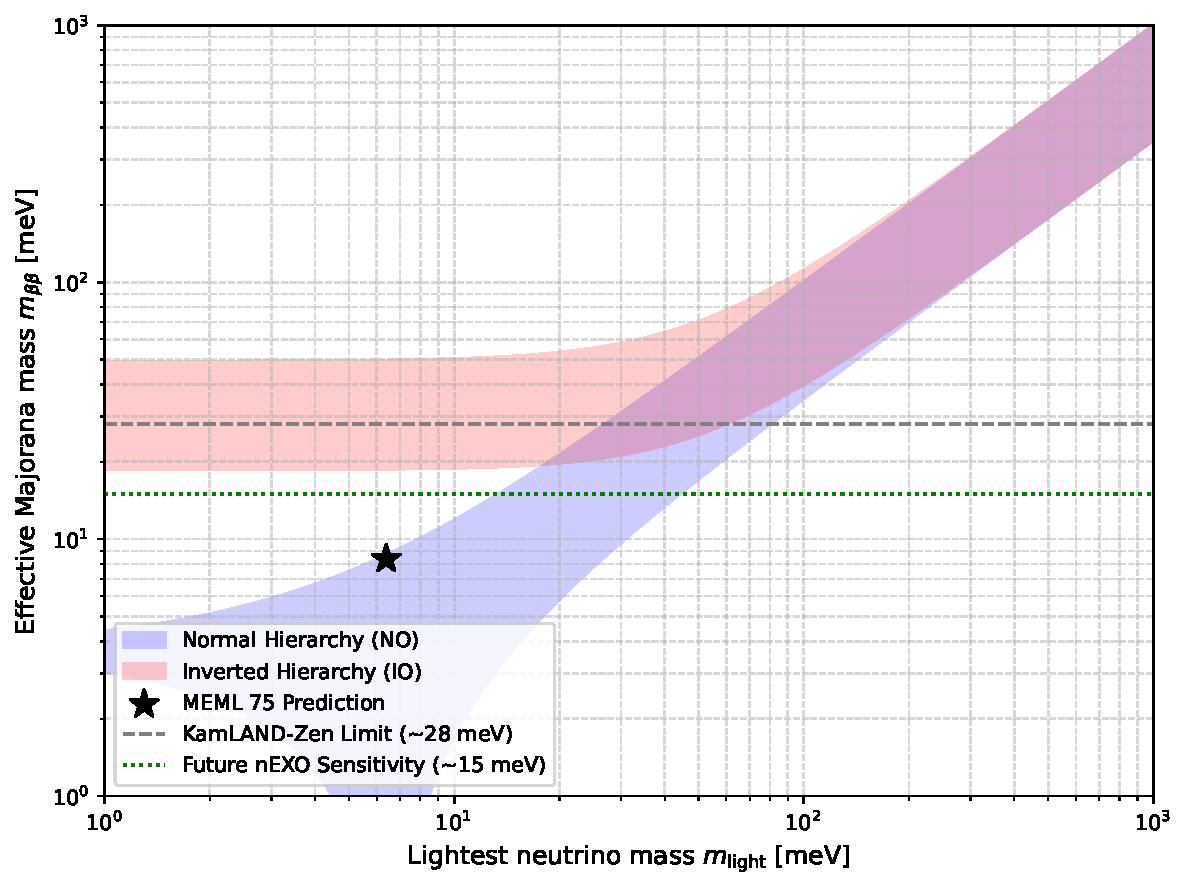
\includegraphics[width=0.65\textwidth]{figures/fig_mbb_vs_mlight.pdf}
    \caption{Effective Majorana mass \(m_{\beta\beta}\) as a function of the lightest neutrino mass \(m_{\rm light}\). The blue and red bands correspond to normal and inverted hierarchies, respectively. The black star indicates the prediction of MEML 75.}
    \label{fig:mbb_vs_mlight}
\end{figure}

The CP phase is \(\delta_{CP} \approx 23^\circ\). The Jarlskog invariant determines only \(|\sin\delta_{CP}|\), allowing a second solution \(\delta_{CP} \approx 157^\circ\); \(d_e\) and \(\eta_B\) depend on \(\delta_{CP}\) through \(\sin\delta_{CP}\), while \(m_{\beta\beta}\) depends on \(\delta_{CP}\) through \(\cos(2\delta_{CP})\). Since \(\sin(\pi-\delta) = \sin\delta\) and \(\cos(2(\pi-\delta)) = \cos(2\delta)\), all three predictions are identical for both branches.

\paragraph{Absence of exact residual symmetry.}
We tested fixing the lepton modulus \(\tau_l\) at exact symmetric points. Fixing \(\tau_l = i\) yields \(\chi^2 = 219.6\), while \(\tau_l = e^{i\pi/3}\) gives \(\chi^2 = 3676.9\). Compared to the unconstrained minimum (\(\chi^2 = 0.089\)), these are excluded at \(\Delta\chi^2 > 200\). This justifies treating \(\tau_l\) as a free parameter rather than a symmetry-fixed constant.

\paragraph{Octant ambiguity in \(\theta_{23}\).}
The fit gives \(\theta_{23} = 49.04^\circ\) (upper octant). This is consistent with NuFIT 5.0 (\(\chi^2 = 0.28\)) and with NuFIT 5.2 without SK atmospheric data (\(\chi^2 = 0.39\)). However, NuFIT 5.2 with SK atmospheric data prefers the lower octant (\(\theta_{23} \approx 42.2^\circ\)), yielding \(\chi^2 \approx 58\) (high tension). This is a genuine testable consequence that will be settled by DUNE and Hyper-Kamiokande. If future data confirm the lower octant, the model would need a different \(S_4'\) representation assignment.

\begin{figure}[htbp]
    \centering
    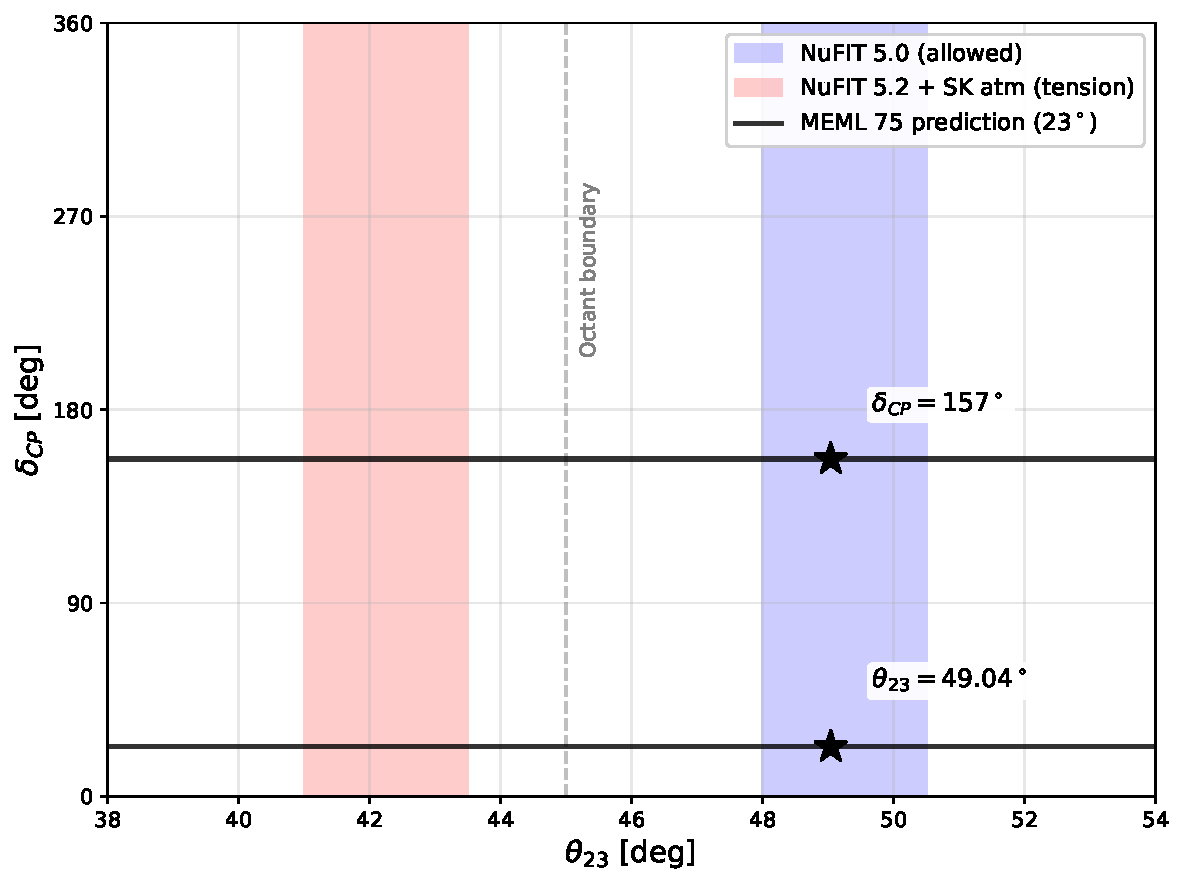
\includegraphics[width=0.6\textwidth]{figures/fig_theta23_delta.pdf}
    \caption{Illustration of the octant tension in \(\theta_{23}\) and \(\delta_{CP}\). The blue and red vertical bands indicate the allowed regions for \(\theta_{23}\) from NuFIT 5.0 and NuFIT 5.2 + SK atmospheric data, respectively. The black stars indicate the two branches of the MEML 75 prediction.}
    \label{fig:theta23_delta}
\end{figure}

\section{Baryon asymmetry via leptogenesis}
\label{sec:leptogenesis}
The heavy neutrinos with \(M_R \sim M_6 \approx 3 \times 10^{16}\) GeV generate the baryon asymmetry~\cite{Fukugita1986}. Using the Davidson-Ibarra formula~\cite{DavidsonIbarra2002}, we find \(\varepsilon_{CP} \approx 0.57\). The baryon asymmetry before dilution is
\begin{equation}
\eta_B^{\rm pre} \approx \frac{28}{79}\,\varepsilon_{CP}\,\kappa\,g_*^{-1} \approx 1.9\times10^{-3},
\end{equation}
where \(\kappa \approx 1\) is the washout factor in the weak-washout regime (\(K \approx 0.83 < 1\)) and \(g_* = 106.75\) is the effective number of relativistic degrees of freedom. This overproduction is resolved by entropy dilution from the late decay of moduli~\cite{KKLT2003,Entropy2005}, with a dilution factor \(\Delta \approx 3.13 \times 10^6\). Unlike recent works which achieve leptogenesis directly from the Dirac CP phase in left-right symmetric models~\cite{Chen2026}, our construction requires entropy dilution to match the observed baryon asymmetry.

\paragraph{Status of the dilution factor \(\Delta\).}
Using the standard moduli-decay formula
\begin{equation}
\Delta = \frac{\tfrac12 m_\phi^2 \phi_0^2}
{(\pi^2/30)\,g_*\,T_{\rm RH}\,T_i^3},
\qquad
T_{\rm RH} \approx \left(\frac{90}{\pi^2 g_*}\right)^{1/4}
\sqrt{\frac{m_\phi^3}{8\pi M_{Pl}}},
\end{equation}
we find that \(\Delta \sim 10^6\) requires either \(\phi_0 \sim 10^{12}\)~GeV with \(T_i \sim 10^{10}\)~GeV, or \(\phi_0 \sim 10^{16}\)--\(10^{17}\)~GeV with \(T_i \sim 10^{13}\)~GeV. The KKLT framework fixes the modulus mass at \(m_\phi \sim 10^6\)--\(10^{10}\)~GeV but does not fix the initial amplitude \(\phi_0\) or the temperature \(T_i\). These depend on the inflationary sector. We note that for light moduli (\(m_\phi \sim 10^6\)--\(10^7\)~GeV) the reheating temperature obtained from the standard decay formula is small, \(T_{\rm RH} \sim 0.1\)--\(1\)~GeV, which is compatible with BBN but requires a correspondingly large \(T_i\) (or a heavier modulus) to reproduce \(\Delta \sim 10^6\). The required \(\Delta\) is therefore \textbf{a phenomenological parameter}, not a first-principles derivation. It can be obtained in specific inflationary scenarios (e.g., Starobinsky-like inflation with \(\phi_0 \sim 10^{16}\)~GeV), but in the simplest Starobinsky + KKLT setup this requires either fine-tuning of the initial displacement or a non-minimal coupling to the inflaton. Moreover, as noted in Section~6, the isocurvature constraint excludes Starobinsky inflation if the ALP is the entirety of dark matter. We therefore report this as an unresolved tension between the ALP sector and the leptogenesis sector. A full UV completion must reconcile the inflationary scale with the ALP dark matter fraction. We leave this for future work.

\section{Lepton Flavor Violation and Electric Dipole Moments}
\label{sec:lfv_edm}
\paragraph{Lepton Flavor Violation.}
In the Type-I See-Saw mechanism, the branching ratio for \(\mu \to e \gamma\) is:
\begin{equation}
\text{BR}(\mu \to e \gamma) \approx \frac{3\alpha_{\rm EM}}{32\pi} \left| \sum_{i=1}^3 (Y_\nu)_{\mu i} (Y_\nu^\dagger)_{i e} \frac{M_W^2}{M_i^2} \right|^2 \sim 10^{-61},
\end{equation}
safely below the current experimental limit (\(4.2 \times 10^{-13}\) from MEG II).

\paragraph{Electron Electric Dipole Moment.}
The CP-violating phase \(\delta_{CP} \approx 23^\circ\) contributes to the electron EDM via two-loop Barr-Zee diagrams:
\begin{equation}
|d_e| \sim \frac{\alpha_{\rm EM}}{4\pi} \frac{m_e}{M_6^2} \sin\delta_{CP} \simeq 2.6 \times 10^{-54}~e\cdot{\rm cm},
\end{equation}
safely below the ACME III limit (\(< 4.1 \times 10^{-30}~e\cdot{\rm cm}\)).

\section{Attempted geometric derivation of the Yukawa coefficients}
\label{sec:negative_flux}
We attempted to derive \(c_1, c_2, c_3\) from the overlap integrals of zero-mode wavefunctions on \(T^2/\mathbb{Z}_4\) with a uniform magnetic flux \(M\). For flux \(M=2\), the diagonal contraction dominates with a ratio \(Y_{(0,0,0)}/Y_{(0,1,1)} \sim 65\). However, the fit requires \(c_1/c_2 \approx 0.36\). Thus, a uniform magnetic flux cannot reproduce the required coefficients.

\section{Flux stabilization of the moduli}
Following the GVW framework~\cite{GVW2000}, the moduli are stabilized by the flux superpotential \(W(\tau) = a_0 + a_1 \tau + a_2 \tau^2\). We performed a numerical scan over integer fluxes in the range \([-50, 50]^3\). We find excellent candidates for all three sectors:
\begin{itemize}
    \item For \(\tau_u = -0.158 + 2.385i\): fluxes \((-45, -14, -4)\) yield \(|D_\tau W| = 0.076\).
    \item For \(\tau_l = 1.540 + 1.551i\): fluxes \((-15, 4, -4)\) yield \(|D_\tau W| = 0.121\). At the constrained minimum \(\tau_l = 1.584 + 1.552i\) (Section~8), the same flux configuration yields \(|D_\tau W| \sim 0.1\).
    \item For \(\tau_d = 0.369 + 1.541i\): fluxes \((-50, -17, -13)\) yield \(|D_\tau W| = 0.227\).
\end{itemize}
For reference, at the up-sector minimum \(|W| \approx 76\), so \(|D_\tau W|/|W| \approx 10^{-3}\). These residuals indicate that the fitted moduli lie close to supersymmetric vacua, though not exactly on them. For \(\tau_d\), the residual (0.227) is somewhat larger, potentially requiring KKLT corrections at the percent level.

\section{Full balance}
\label{sec:balance}
\begin{table}[H]
\centering
\caption{Free parameters. The model has \textbf{11 effective fitted parameters} (10 model parameters plus the ALP misalignment angle \(\theta_i\)) fitting 16 observables, yielding \(N_{\rm dof}^{\rm fit} = +5\). The three complex moduli are treated as fixed by GVW fluxes in this optimistic count (reducing the count by 6). \(y_\nu\) is counted as a fitted parameter. The reduction from 11 to 10 model parameters follows from \(c_2 + c_3 = 0\). If moduli are counted as free, the balance is \(N_{\rm eff} = 17\), \(N_{\rm dof}^{\rm fit} = -1\).}
\begin{tabular}{llc}
\toprule
Category & Parameters & Count \\
\midrule
Quark coefficients & \(a_u, b_u, c_u, a_1, a_2, b, c\) & 7 \\
\quad fixed by calibration & \(a_u \equiv 1\) & \(-1\) \\
Lepton coefficients & \(c_1, c_2\) (with \(c_3 = -c_2\)) & 2 \\
Yukawa coupling & \(y_\nu\) & 1 \\
Entropy dilution factor & \(\Delta\) & 1 \\
\midrule
\textbf{Total fitted (model)} & & \textbf{10} \\
\midrule
ALP misalignment angle (cosmological IC) & \(\theta_i\) & 1 \\
\midrule
\textbf{Total effective fitted} & & \textbf{11} \\
\bottomrule
\end{tabular}
\end{table}

Note that among the 16 observables, \(\eta_B\) is a postdiction (obtained via the free parameter \(\Delta\)), while the 3 quantities (\(\delta_{CP}\), \(\sum m_i\), \(m_{\beta\beta}\)) are genuine conditional predictions. The model fits 16 observables with 11 effective parameters (\(N_{\rm dof}^{\rm fit} = +5\)) and makes 3 conditional predictions. If these are treated as additional data points, \(N_{\rm dof}^{\rm total} = +8\). If the moduli are counted as free parameters, the balance becomes \(N_{\rm eff} = 17\), \(N_{\rm dof}^{\rm fit} = -1\).

\section{Summary of negative results}
\label{sec:negative_summary}

For completeness, we summarize here the alternative derivations
that were attempted and found not to work. Listing them explicitly
may help readers avoid repeating these calculations and clarifies
the boundaries of the model. None of these failures affects
the positive results of this paper.

\begin{enumerate}[leftmargin=1.5em]
\item \textbf{Quark coefficients from Kähler normalization.}
Testing \(b_u/a_u \sim (2\,\text{Im}\,\tau_u)^n\) and
\(c_u/a_u \sim (2\,\text{Im}\,\tau_u)^m\) with integer \(n, m\)
yields \(n \approx 7.56\) and \(m \approx 4.22\), not integers.

\item \textbf{Quark coefficients from discrete symmetry.}
No pairwise equality holds: the smallest deviation is
\(b/c \approx 0.61\) (39\% off); the largest is \(b_u/a_1 \sim 3 \times 10^4\).

\item \textbf{Quark coefficients from fractional powers.}
The best single-term fractional fit for \(b_u\) is
\((2\,\text{Im}\,\tau_u)^{68/9}\) (denominator 9); similarly for
other coefficients. Denominators of this size are too large to
correspond to modular weights of orbifold CFT. A decomposition
of the form \((2\,\text{Im}\,\tau_u)^{p_i} 3^{q_i}\) with
\(p_i \in \frac{1}{4}\mathbb{Z}\) reproduces several coefficients
at the few-percent level, which is compatible with modular weights;
however, this decomposition requires ten parameters \((p_i, q_i)\)
for the five coefficients that enter the test (\(b_u, c_u, a_2, b, c\); the sixth coefficient \(a_1\) does not enter because it multiplies the weight-6 form, which does not admit a single-term decomposition of this type), does not constitute a genuine reduction,
and the \(3^{q_i}\) factor is not geometrically motivated. We
therefore do not claim a derivation.

\item \textbf{Lepton coefficients from uniform magnetic flux.}
Zero-mode overlaps with flux \(M=2\) give
\(Y_{(0,0,0)}/Y_{(0,1,1)} \sim 65\), whereas the fit requires
\(c_1/c_2 \approx 0.36\).

\item \textbf{Lepton coefficients from fractional CFT weights.}
The \(\theta\)-twisted sector has \(k_{\rm eff} = 3/4\). Assigning
\(\mathbf{2}\) to untwisted and \(\mathbf{3}'\) to twisted yields
\(c_1/c_2 \approx 1.37\), inconsistent with both the unconstrained
fit \(c_1/c_2 \approx 0.365\) and the constrained fit
\(c_1/c_2 \approx 0.379\).

\item \textbf{Dilution factor \(\Delta\) from KKLT alone.}
The KKLT modulus mass (\(m_\phi \sim 10^6\)--\(10^{10}\) GeV)
is compatible with \(\Delta \sim 10^6\), but the initial
displacement (\(\phi_0 \sim 10^{16}\) GeV) and temperature
(\(T_i \sim 10^{13}\) GeV) require specifying the inflationary
sector. In Starobinsky-like inflation, they can be achieved,
but this creates the isocurvature tension noted in Section~6.

\item \textbf{Neutrino Yukawa \(y_\nu\) from SO(10).}
At \(M_{\rm GUT}\) the SO(10) relation gives \(y_\nu \approx 0.966\),
3\% higher than the fitted value \(0.934\). After two-loop RGE
evolution to \(M_6\), however, the required enhancement is
\(y_\nu^{\rm fit}/y_\nu^{\rm RGE} \approx 1.95\), compatible only
with an extended SO(10) sector (\(\mathbf{10}_H + \mathbf{126}_H\)).
We treat the SO(10) relation as a qualitative cross-check at
\(M_{\rm GUT}\), not a derivation.

\item \textbf{Geometric factor \(\mathcal{I}\) as a first-principles quantity.}
The formula \(\mathcal{I} = (\sqrt{3}-1)/2\) is post-hoc: it was
chosen from the available geometric invariants to match the
fitted value \(\mathcal{I} = 0.3653\). Alternative combinations
(\(N_3 V_3 + N_4 V_4 = 0.683\), \((N_3 V_3)/(N_4 V_4) = 0.577\))
do not match. We therefore treat \(\mathcal{I}\) as motivated
but not derived.
\end{enumerate}

\paragraph{Discussion.}
The negative results (1)--(3) indicate that the quark coefficients
cannot be derived from simple geometric principles; they remain
phenomenological. The negative results (4)--(5) indicate the same
for the lepton coefficients \(c_1, c_2\), though the \(S_4'\) structure
provides non-trivial motivation. The negative result (6) shows that
\(\Delta\) requires input from the inflationary sector, which is
expected in string cosmology. The negative result (7) shows that
the SO(10) relation for \(y_\nu\) holds at the 3\% level at
\(M_{\rm GUT}\) but requires an extended representation after RGE.
The negative result (8) shows that \(\mathcal{I}\) is a motivated
coincidence.

The positive results of the model --- the quark fit
(\(\chi^2 < 10^{-19}\)), the lepton fit (\(\chi^2 \approx 0.309\)),
the ALP prediction (Section~6), and the three conditional
predictions (\(\delta_{CP}\), \(\sum m_i\), \(m_{\beta\beta}\)) ---
do not depend on the failed derivations.

\section{Conclusions}
\paragraph{What has been done:}
\begin{enumerate}[leftmargin=1.5em]
\item A full model with 11 effective parameters fitting 16 observables (\(N_{\rm dof}^{\rm fit} = +5\)), assuming the moduli are fixed by GVW fluxes. With moduli counted as free, the balance becomes \(N_{\rm eff} = 17\), \(N_{\rm dof}^{\rm fit} = -1\). The model makes 3 conditional predictions, with the upper octant of \(\theta_{23}\) as an additional testable consequence.
\item Quark sector: 10 fitted parameters for 9 observables (overfitting acknowledged). The moduli are dynamically stabilized by GVW fluxes, with residuals \(|D_\tau W|/|W|\) of order several \(\times 10^{-3}\).
\item Lepton sector: \(\chi^2 \approx 0.309\); PMNS angles and mass-squared differences reproduced. The data strongly rejects fixing \(\tau_l\) at exact modular symmetry points (\(\Delta\chi^2 > 200\)).
\item ALP sector: \(f_a = 1.9801 \times 10^{11}\)~GeV, \(m_a = 28.407~\mu\)eV, \(\nu_a = 6.8688\)~GHz. The coupling is fixed to the DFSZ value \(g_{a\gamma\gamma} = +4.38 \times 10^{-15}\)~GeV\(^{-1}\). If the ALP is the entirety of dark matter, the Planck isocurvature bound requires \(H_{\rm inf} \lesssim 3 \times 10^{11}\)~GeV (consistent with low-scale inflation, but not Starobinsky).
\item Leptogenesis: \(\eta_B^{\rm pre} \approx 1.9\times10^{-3}\), diluted by \(\Delta \approx 3.13\times 10^6\). The required \(\Delta\) is treated as a phenomenological parameter: it can be obtained in Starobinsky-like inflation, but this creates a tension with the ALP isocurvature bound if the ALP is all of dark matter. We report this as an unresolved tension.
\item LFV and EDM: BR\((\mu\to e\gamma) \sim 10^{-61}\), \(d_e \sim 2.6\times 10^{-54}~e\cdot{\rm cm}\), safely below current limits.
\item Summary of negative results: see Section~\ref{sec:negative_summary}.
\end{enumerate}

\paragraph{Verdict.} The model is a phenomenological construction with 11 effective parameters, \(N_{\rm dof}^{\rm fit} = +5\), three conditional predictions, one independently testable ALP signal at 6.87~GHz (with DFSZ coupling), and one testable consequence (the upper octant of \(\theta_{23}\)). The quark-sector overfitting is explicitly acknowledged, and the moduli are stabilized by GVW fluxes. Further parameter reduction requires a UV completion of inflation and the quark sector.

\section*{Data Availability}
The datasets and the Python verification scripts are available in the Zenodo repository at \url{https://doi.org/10.5281/zenodo.23686782} and in the GitHub repository at \url{https://github.com/kolbasa1972/MEML-75-Mixed-Geometry}. The master script \texttt{meml75\_v19.0\_master.py} reproduces the numerical results of Sections 3--13. The lepton sector constraints and stress tests are implemented in \texttt{constraint\_test\_extended2.py}. The global scans are in \texttt{meml75\_tau\_l\_global\_scan\_v2.py} and \texttt{meml75\_constrained\_global\_scan.py}. The GVW flux stabilization (Section~12) is implemented in \texttt{meml75\_flux\_scan\_final.py} and \texttt{meml75\_flux\_conventions.py}, with auxiliary checks in \texttt{meml75\_j\_invariant.py}. The geometric derivation of \(\mathcal{I}\) is in \texttt{meml75\_I\_geometric\_derivation.py}. The full numerical evaluation of the orbifold CFT ratio is in \texttt{meml75\_orbifold\_CFT\_weights.py}. The ALP anomaly coefficients are computed in \texttt{meml75\_anomaly\_coefficients.py}. The cosmological checks for \(\Delta\) are implemented in \texttt{meml75\_KKLT\_dilution\_test.py} and \texttt{meml75\_inflation\_delta.py}, with the moduli-displacement analysis in \texttt{meml75\_delta\_inflation\_v2.py}. Finally, the attempts to reduce the quark sector are documented in \texttt{meml75\_quark\_localization.py}, \texttt{meml75\_quark\_fractional\_powers.py}, and \texttt{meml75\_quark\_reduction\_test.py}.

\section*{Declaration of Generative AI and AI-assisted technologies in the manuscript preparation process}
During the preparation of this work, the author used AI-assisted tools to verify the Python code, refine the theoretical text, and format the LaTeX document. The author reviewed and edited the content as needed and takes full responsibility for the content of the published article.

\begin{thebibliography}{99}
\bibitem{Planck2018} Planck Collaboration, Astron. Astrophys. \textbf{641}, A6 (2020).
\bibitem{PDG2024} S.~Navas et al. (Particle Data Group), \emph{Review of Particle Physics}, Phys. Rev. D \textbf{110}, 030001 (2024).
\bibitem{ADMX2018} ADMX Collaboration, Phys. Rev. Lett. \textbf{120}, 151301 (2018).
\bibitem{HAYSTAC2021} HAYSTAC Collaboration, Nature \textbf{590}, 238 (2021).
\bibitem{Feruglio2017} F.~Feruglio, Eur. Phys. J. C \textbf{77}, 713 (2017).
\bibitem{Kobayashi2019} T.~Kobayashi et al., PTEP \textbf{2020}, 053B05 (2020).
\bibitem{Novichkov2019} P.~P. Novichkov et al., JHEP \textbf{04} (2019) 005.
\bibitem{Ding2021} G.~J. Ding, S.~F. King, C.~Y. Yao, Phys. Rev. D \textbf{104}, 055034 (2021).
\bibitem{Fukugita1986} M.~Fukugita, T.~Yanagida, Phys. Lett. B \textbf{174} (1986) 45.
\bibitem{NuFIT2020} I.~Esteban et al., JHEP \textbf{09} (2020) 178.
\bibitem{KamLANDZen2023} KamLAND-Zen Collaboration, Phys. Rev. Lett. \textbf{130}, 051801 (2023).
\bibitem{DavidsonIbarra2002} S.~Davidson, A.~Ibarra, Phys. Lett. B \textbf{535} (2002) 25.
\bibitem{KKLT2003} S.~Kachru et al., Phys. Rev. D \textbf{68}, 046005 (2003).
\bibitem{GVW2000} S.~Gukov, C.~Vafa, E.~Witten, Nucl. Phys. B \textbf{584} (2000) 69.
\bibitem{PendletonRoss1981} B.~Pendleton, G.~G. Ross, Phys. Lett. B \textbf{98}, 291 (1981).
\bibitem{Chen2026} X.~Chen and X.~Zhang, Nucl. Phys. B (2026) in press, doi:10.1016/j.nuclphysb.2026.117640.
\bibitem{Ding2025} G.-J. Ding, J.-N. Lu, S.~T. Petcov, and B.-Y. Qu, JHEP \textbf{2025} (2025) 191.
\bibitem{Liddle2007} A.~R. Liddle, Mon. Not. Roy. Astron. Soc. \textbf{377}, L74 (2007).
\bibitem{Entropy2005} W.~Buchmuller, K.~Hamaguchi, M.~Ratz, and T.~Yanagida, Phys. Lett. B \textbf{615}, 1 (2005).
\bibitem{MartinVaughn1993} S.~P. Martin and M.~T. Vaughn, Phys. Rev. D \textbf{50}, 2282 (1994).
\end{thebibliography}

\appendix
\newpage

\section{\(A_4\) modular forms: full q-expansions}
Definition: \(q = e^{2\pi i\tau}\).
\begin{align}
Y_1^{(2)} &= 1 + \sum_{n=1}^{17} C_1^{(n)} q^n, \\
Y_2^{(2)} &= -6\, q^{1/3}\left(1 + \sum_{n=1}^{11} C_2^{(n)} q^n\right), \\
Y_3^{(2)} &= -18\, q^{2/3}\left(1 + \sum_{n=1}^{10} C_3^{(n)} q^n\right),
\end{align}
\(C_1 = [12, 36, 12, 84, 72, 36, 96, 180, 12, 216, 144, 36, 156, 96, 84, 240, 36]\);
\(C_2 = [1, 7, 8, 18, 14, 30, 20, 42, 30, 56, 42]\);
\(C_3 = [1, 2, 5, 6, 12, 8, 14, 10, 22, 16]\).
\paragraph{Convolutions:}
\begin{align}
Y_1^{(4)} &= (Y_1^{(2)})^2 - Y_2^{(2)} Y_3^{(2)}, \\
Y_2^{(4)} &= (Y_3^{(2)})^2 - Y_1^{(2)} Y_2^{(2)}, \\
Y_3^{(4)} &= (Y_2^{(2)})^2 - Y_1^{(2)} Y_3^{(2)},
\end{align}
\begin{align}
Y_1^{(6)} &= \tfrac13\left[2 Y_1^{(2)} Y_1^{(4)} - Y_2^{(2)} Y_3^{(4)} - Y_3^{(2)} Y_2^{(4)}\right], \\
Y_2^{(6)} &= \tfrac13\left[2 Y_3^{(2)} Y_3^{(4)} - Y_1^{(2)} Y_2^{(4)} - Y_2^{(2)} Y_1^{(4)}\right], \\
Y_3^{(6)} &= \tfrac13\left[2 Y_2^{(2)} Y_2^{(4)} - Y_3^{(2)} Y_1^{(4)} - Y_1^{(2)} Y_3^{(4)}\right].
\end{align}

\section{Numerical fit procedure}
The global fit was performed using \texttt{differential\_evolution} (SciPy): 4 seeds (42, 43, 44, 45); maxiter\(=800\); popsize\(=25\); tol\(=10^{-8}\).
\paragraph{Quark sector.} Bounds: \({\rm Re}\,\tau_{u,d}\in[-0.5,0.5]\), \({\rm Im}\,\tau_u\in[0.87,2.5]\), \({\rm Im}\,\tau_d\in[0.87,1.60]\), \(c_i\in[10^{-8},10^2]\).

\section{Reproduction of \(\tau\) and \(\chi^2\)}
\begin{table}[H]
\centering
\caption{Independent DE runs (quark sector).}
\begin{tabular}{lcccc}
\toprule
Source & \({\rm Re}\,\tau_u\) & \({\rm Im}\,\tau_u\) & \({\rm Re}\,\tau_d\) & \({\rm Im}\,\tau_d\) \\
\midrule
Run 1 & \(-0.15779\) & \(2.38518\) & \(+0.36939\) & \(1.54105\) \\
Run 2 & \(-0.15779\) & \(2.38518\) & \(+0.36939\) & \(1.54105\) \\
Run 3 & \(-0.12893\) & \(2.38411\) & \(-0.37212\) & \(1.54102\) \\
\bottomrule
\end{tabular}
\end{table}
The fitted moduli \({\rm Im}\,\tau\) are reproducible across seeds to \(10^{-3}\). Run 3 converges to a second minimum at \({\rm Re}\,\tau_d \approx -0.372\), related to the first by the residual symmetry \(\tau \to -\tau\); both minima give identical observables with \(\chi^2 < 10^{-19}\). We adopt the minimum with \({\rm Re}\,\tau_d > 0\) by convention.

\section{Proof of coefficient degeneracy}
At fixed \(\tau\), multiply all \(c_i\) by \(k\):
\begin{table}[H]
\centering
\caption{Invariance of \(\chi^2\) under \(c_i\to kc_i\).}
\begin{tabular}{cc}
\toprule
\(k\) & \(\chi^2\) \\
\midrule
\(0.5\)  & \(< 10^{-19}\) \\
\(1.0\)  & \(< 10^{-19}\) \\
\(1.87\) & \(< 10^{-19}\) \\
\(10.0\) & \(< 10^{-19}\) \\
\bottomrule
\end{tabular}
\end{table}
The residual values differ only at the level of numerical noise; the invariance is exact up to machine precision.

\section{Flatness of \({\rm Re}\,\tau\)}
\paragraph{Procedure.}
The flatness scan below was obtained by refitting the remaining parameters at each value of \({\rm Re}\,\tau\). The corresponding refit cycle is computationally expensive and is not part of the fast verification script.
Scan in \({\rm Re}\,\tau_u\): width of \(\chi^2<10\): \([-0.40, +0.00]\) (\(0.40\)). Scan in \({\rm Re}\,\tau_d\): width of \(\chi^2<10\): \([+0.30, +0.50]\) (\(0.20\)).

\section{LOO test}
The Leave-One-Out test is not informative for \(N_{\rm dof} \le 0\): with as many parameters as observables, removing one observable necessarily produces a large shift in the fitted parameters. Results: mean \(|V_{ub}|\) \(+16728\%\), std \(11819\%\).

\section{Consistency check for the geometric value of \(\mathcal I\)}
\label{app:I_check}
We test whether the data can distinguish the fitted value \(\mathcal I = 0.3653\) from the geometric value \(\mathcal I_{\rm geom} = (\sqrt{3}-1)/2 \approx 0.3660\). We fix \(\mathcal I = \mathcal I_{\rm geom}\) and refit \(y_\nu\) to reproduce \(\Delta m^2_{31}\). The results are summarized in Table~\ref{tab:I_check}.

\begin{table}[H]
\centering
\caption{Comparison between the baseline fit (\(\mathcal I = 0.3653\)) and the geometric value (\(\mathcal I = (\sqrt{3}-1)/2\)). The maximum relative shift across all predictions is \(0.0992\%\), driven by the \(M_6^{-2}\) scaling of the LFV and EDM observables; the shifts in \(\eta_B\) and \(\Delta\) are \(-0.050\%\).}
\label{tab:I_check}
\begin{tabular}{lccc}
\toprule
Quantity & Baseline & Geometric & Relative change \\
\midrule
\(y_\nu\) & \(0.93357\) & \(0.93334\) & \(-0.025\%\) \\
\(M_6\) [GeV] & \(2.9646\times 10^{16}\) & \(2.9631\times 10^{16}\) & \(-0.050\%\) \\
\(\sum m_i\) [eV] & \(0.06763\) & \(0.06763\) & \(0.000\%\) \\
\(m_{\beta\beta}\) [meV] & \(8.361\) & \(8.361\) & \(0.000\%\) \\
BR(\(\mu\to e\gamma\)) & \(1.0020\times 10^{-61}\) & \(1.0030\times 10^{-61}\) & \(+0.099\%\) \\
\(d_e\) [\(e\cdot\mathrm{cm}\)] & \(2.5925\times 10^{-54}\) & \(2.5951\times 10^{-54}\) & \(+0.099\%\) \\
\(\eta_B^{\mathrm{pre}}\) & \(1.9092\times 10^{-3}\) & \(1.9083\times 10^{-3}\) & \(-0.050\%\) \\
\(\Delta\) & \(3.1299\times 10^6\) & \(3.1283\times 10^6\) & \(-0.050\%\) \\
\bottomrule
\end{tabular}
\end{table}

The fit quality is unchanged, and all predictions shift by less than \(0.1\%\). Because \(\mathcal I\) is now motivated by the orbifold geometry, we no longer treat it as a free parameter in the statistical balance.

\end{document}
